\documentclass[../main]{subfiles}
\begin{document}

\section{
  \cpp language constructs for metaprogramming
}
\label{lbl:cpp-meta-constructs}

\cpp templates are an interesting feature for metaprogramming. As they
are Turing-complete \cite{unruh:1994}, one can design a set of
\textbf{template metaprograms} \cite{abrahams:2004} that allow the compiler
to perform arbitrary computation at compile time, and generate
\cpp code fragments as an output.
The resulting source code is then merged with the rest of the program
and processed through the subsequent compilation stages.

Due to the fact that templates are instantiated at compile-time, they can only
accept types and compile-time constants as parameters. Templates support
pattern-matching and recursion thanks to partial template specialization,
making it equivalent to a pure functional language \cite{haeri:2012}.

This complex logic is often used to implement \gls{hpc} libraries that embed
high level declarative languages based on \cpp's syntax, and provide
high performance portable functionalities thanks to metaprogramming.

\subsection{
  \cpp template metaprogramming
}

Listing \ref{lst:basic-tmp} shows basic principles of \cpp template
metaprogramming. The \lstinline{fibonacci_t} type template accepts an
integer called $N$, and exposes the $N\textsuperscript{th}$ element
of the Fibonacci series as its \lstinline{value} static member.
The template has 3 definitions:
a generic one to calculate elements for $N > 1$,
and two specializations for elements of ranks $0$ and $1$.

\begin{lstlisting}[
  language=C++,
  caption=Fibonacci series computation using C++ templates,
  label=lst:basic-tmp
]{}
template <unsigned N> struct fibonacci_t;

template <unsigned N> struct fibonacci_t {
  static constexpr unsigned value =
      fibonacci_t<N - 2>::value +
      fibonacci_t<N - 1>::value;
};

// Specializations for cases 0 and 1
template <> struct fibonacci_t<0> {
  static constexpr unsigned value = 0;
};

template <> struct fibonacci_t<1> {
  static constexpr unsigned value = 1;
};

std::array<int, fibonacci_t<5>::value> some_array;
\end{lstlisting}

Note that template parameters in \ref{lst:basic-tmp} are values and not types.
This is allowed since \cpp11 as \glspl{nttp} were introduced along with
the \textbf{\gls{constexpr}} function and variable qualifier.
Before \glspl{nttp} were introduced, even numerical values
had to be represented using types.

The \gls{constexpr} qualifier allows functions and variables to be used to
produce \glspl{nttp}, or more broadly, to be used in \textbf{\glspl{consteval}}.
\Glspl{consteval} are evaluations that result in the creation of
compile-time constants such as \glspl{nttp}.
In this example, the constant is the size of a static array.

This evolution of the \cpp standard marks the beginning of
\textbf{value-based metaprogramming}, in opposition to
\textbf{type-based metaprogramming}. Although in this example, both types
and values are involved in the compile-time computation.

\subsection{
  Different kinds of templates
}

\cpp templates offer ways to output code for data structures, values,
and functions. Ultimately, these kinds outputs constitute what metaprograms
can or cannot generate.

\begin{itemize}

  \item

\textbf{Type templates} to generate data structures.

\begin{lstlisting}[language=c++]{}
template <typename T> struct named_value_t {
  std::string name;
  T value;
};
\end{lstlisting}

  \item

\textbf{Type alias templates} which can be used as abstractions on top of
template types.

\begin{lstlisting}[language=c++]{}
template <typename T>
using nested_named_value_t =
    named_value_t<named_value_t<T>>;
\end{lstlisting}

  \item

\textbf{Function templates} to create generic functions.

\begin{lstlisting}[language=c++]{}
/// Returns a value annotated with
/// its string representation
template <typename T>
named_value_t<T> make_named_value(T value) {
  return named_value_t<T>(std::to_string(value),
                          std::move(value));
}
\end{lstlisting}

  \item

\textbf{Variable templates} to map template parameters to values.

\begin{lstlisting}[language=c++]{}
/// Returns the default value of T annotated with
/// its string representation
template <typename T>
named_value_t<T> annotated_default_v =
    make_named_value(T{});

named_value_t<int> val = annotated_default_v<int>;
\end{lstlisting}

\end{itemize}

\subsection{
  Different kinds of parameters
}

% TODO: Rajouter un exemple pour synthetiser chaque categorie de parametres

Metaprograms can take many kinds of \cpp constructs as inputs.

\begin{itemize}

  \item

\textbf{Type parameters} are the primary kind of parameter used in \gls{tmp}
in which types are used to represent everything from enumerations, arrays,
or even functions.

  \item

\textbf{\glspl{nttp}} are complementary with type parameters.
They can be used to wrap values within types, which can be particularly useful
in the context of \gls{tmp}. For example a type template definition like
\lstinline|template<int I> integer_t{};| allows integers to be stored as types.

  \item

\textbf{Parameter packs} make it possible for templates to have an
arbitrary number of parameters, as long as types and values
are not mixed together. Parameter packs also exist for function parameters,
which can be useful for template parameter deduction.

For example a type template definition like
\lstinline|template<typename ... Ts> tuple_t{};| can be used to store an
arbitrary list of types as a single type.

  \item

\textbf{Regular function parameters} can be used in certain conditions.
Since \cpp11, functions and variables can be qualified as \gls{constexpr}
and used to produce \glspl{nttp}.

\end{itemize}

\subsection{
  Advanced \cpp template mechanisms
}

\begin{itemize}
  \item

\textbf{Template specialization} allows specializing a template for a given
set of type or value parameters. A template that has a single boolean parameter
can, for example, expose two different implementations depending on the
parameter's value.

  \item

\textbf{Template parameter deduction} works as a form of pattern matching
for function template parameters, types and values alike. It can filter
parameter patterns, and deduce nested template parameters in those patterns.

  \item

\textbf{\gls{sfinae}} is a \cpp principle that consists in not triggering a
compilation error when a type substitution cannot be done in a template
instantiation. Instead the type, function, or variable will simply be disabled
and the next candidate will be instantiated.

  \item

\textbf{Parameter pack expansion} allows mapping operations and performing
reductions on parameter packs.

\end{itemize}

\subsection{
  Compile time logic
}

Compile time logic can be achieved in many \cpp constructs.

\begin{itemize}

  \item

\textbf{Computation using types}, also known as type-based metaprogramming.
Types can be used to represent scalar values, arrays, and many more
kinds of data structures including expression trees. They can also

  \item

\textbf{Computation using values} thanks to \glspl{nttp}.
They allow a slightly more explicit way to write metaprograms,
as values are represented by values instead of types.
Not all values are accepted as \gls{nttp}.
Until \cpp20, only integral values (\ie integers, booleans, etc.)
could be used as \gls{nttp}.

  \item

\textbf{Computation using \gls{constexpr} functions} since \cpp11,
although only a limited subset of \cpp can run in \glspl{consteval}.
Memory allocations have been allowed in this context only since \cpp20.

\end{itemize}

The use of \gls{constexpr} functions for compile time programming might be
preferable for many reasons: they are familiar to all \cpp developers
(and, as such, are more maintainable), they allow the use of types to enforce
semantics properly as opposed to type-based metaprogramming, and they allow
compile time programs to run much faster than pure \gls{tmp} does.

% TODO: Rajouter un exemple de fibonacci en fonction constexpr

Metaprogramming is essential to implement high level \glspl{dsel} that translate
into high performance programs through a series of transformations that
occur at compile-time, akin to an additional user-defined compilation stage
embedded into the compilation process itself.

\section{
  Domain specific embedded language
}
\label{lbl:expression-level-metaprogramming}

% By definition, a Domain-Specific Language (DSL) is a computer language special-
% ized to a particular application domain, contrary to a general-purpose language,
% which is broadly applicable across domains, and lacks specialized features for a par-
% ticular domain. Domain Specific Embedded Languages (DSELs) are a subclass of
% DSL that rely on an existing general-purpose language to host it. DSELs then reuse
% the host language syntax and tool ecosystem to be compiled or interpreted. The
% compile-time process of generating new code (either inside or outside the current
% host language) known as Template Meta-Programming is then used to ensure
% performances and correctness.

% TODO: Citer un peu boost.proto

% DEBUT
\glspl{dsel} in \cpp use \gls{tmp} via the \textbf{\gls{et}} idiom.
\glspl{et} \cite{veldhuizen:1995,vandevoorde:2002} is a
technique implementing a form of \textbf{delayed evaluation} in
\cpp \cite{spinellis:2001}. Expression Templates are built around the
\textbf{recursive type composition} idiom \cite{jarvi:1998} that allows the
construction, at compile time, of a type representing the \gls{ast}
of an arbitrary statement. This is done by overloading functions and operators
on those types so they return a lightweight object.
The object encodes the current operation in the \gls{ast}
being built in its type instead of performing any kind of computation.
Once reconstructed, this \gls{ast} can be transformed into arbitrary code fragments
using Template Metaprograms.

As of today, most \cpp \glspl{dsel} rely on \gls{et} and therefore
are limited to the \cpp syntax. New techniques are becoming more popular through
the use of \gls{constexpr} strings to embed arbitray
\glspl{dsel}. One major example is the \gls{ctre} \cite{ctre}
that implements most of the \gls{pcre} syntax.
However, \gls{ctre} still relies on type-based \gls{tmp} to parse
regular expressions and transform them into regular expression evaluators.
% FIN

% TODO: Rajouter exemple CTRE
\begin{lstlisting}[
  language=c++
]{}
struct date {
  std::string_view year;
  std::string_view month;
  std::string_view day;
};

std::optional<date>
extract_date(std::string_view s) noexcept {
  using namespace ctre::literals;
  if (auto [whole, year, month, day] =
          ctre::match<
              "(\\d{4})/(\\d{1,2})/(\\d{1,2})">(
              s);
      whole) {
    return date{year, month, day};
  } else {
    return std::nullopt;
  }
}
\end{lstlisting}

In this section, I will cover the use of \gls{tmp} for higher levels
of abstraction.

\subsection{
  A use case for Expression Templates
}

Combined with compile-time mechanisms such as function overloading,
specialization, and operator overloading, \glspl{et} can be used to
implement expression level \glspl{dsel} and convert complex
mathematical expressions into high performance code\cite{veldhuizen:1995}.
There are two main libraries that are able to do this: Eigen \cite{eigen}
and Blaze \cite{blazelib}.

\begin{figure}[h]
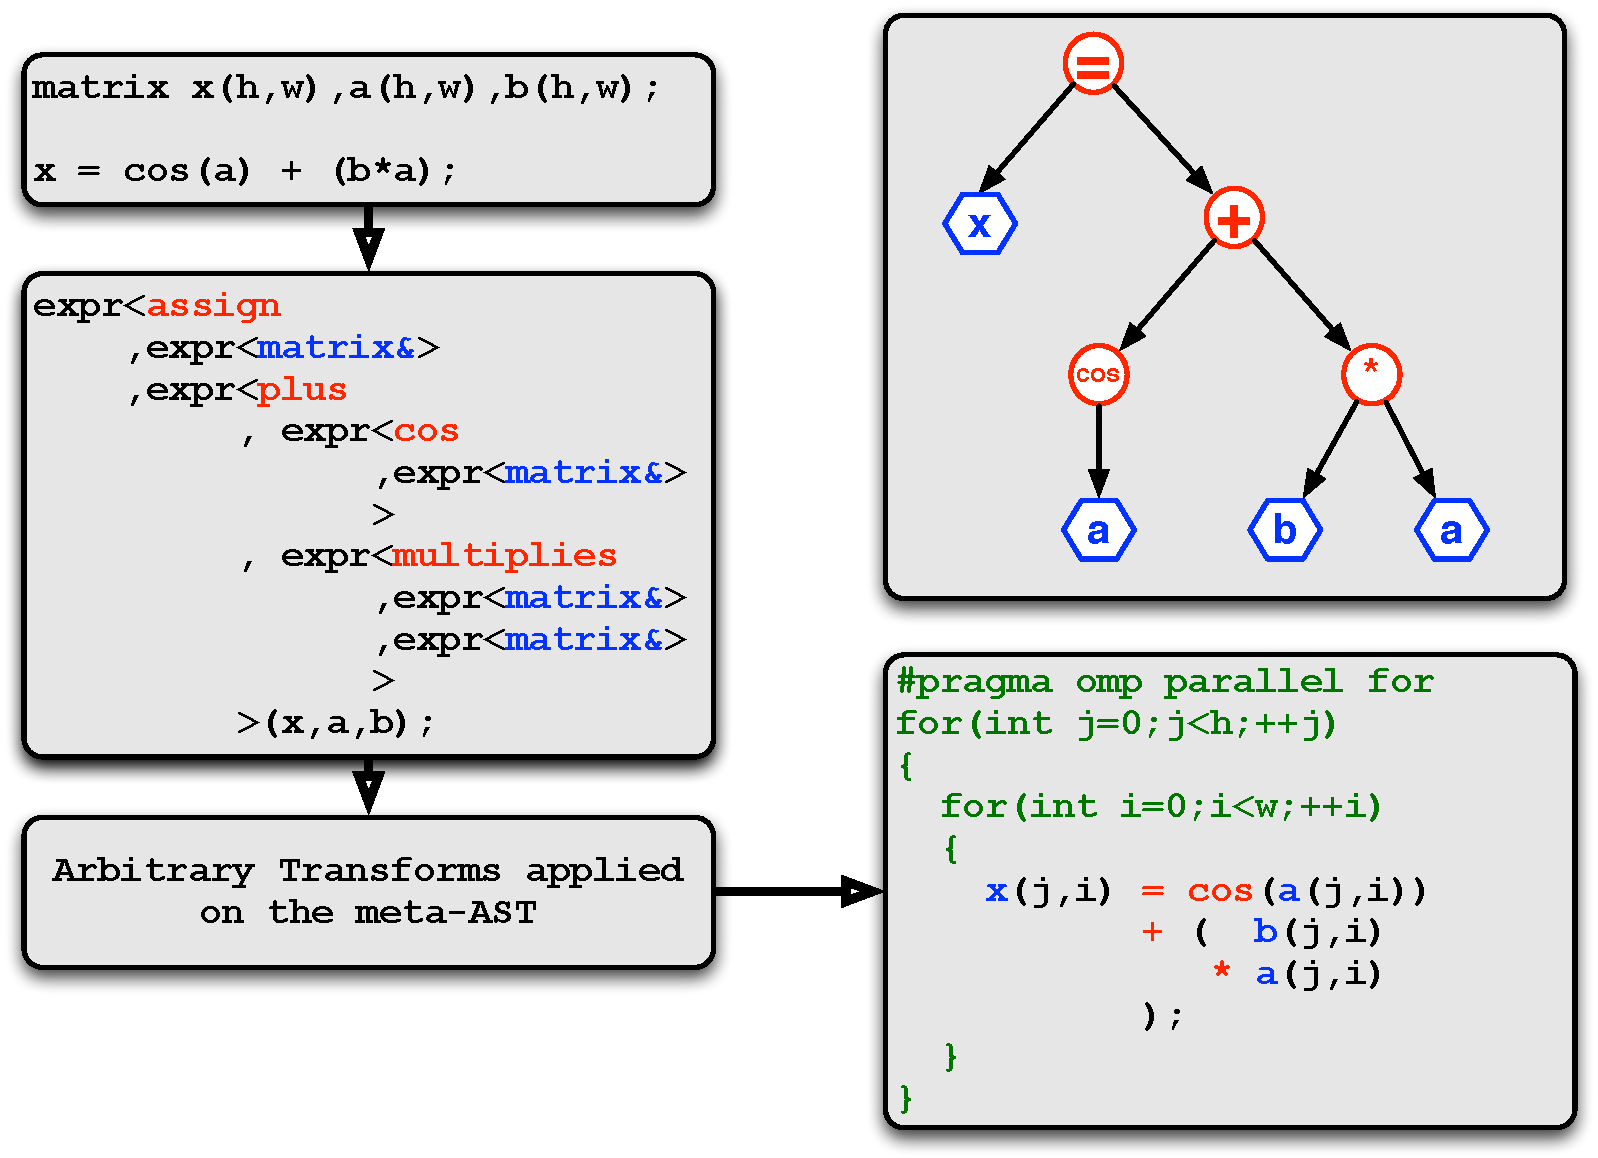
\includegraphics[width=\textwidth]{images/expressiontemplates.pdf}
\caption{
  Expression template evaluation illustration\cite{falcou-hdr}
}
\label{fig:expression-template-illustration}
\end{figure}

Figure \ref{fig:expression-template-illustration} shows how mathematical
expressions can be encoded via \glspl{et}: an operation involving matrices
generates a type hierarchy that represents the operation itself,
and the assignment of this expression to \lstinline{x} triggers the generation
of an optimized program that computes the operation.

They enable a whole range of optimizations:

\begin{itemize}

\item
\textbf{Lazy evaluation} is easily implemented through the generation
of access operators that calculate single element values in one to one
element operations such as additions or substractions.

\item
\textbf{\gls{blas} functions} can be used on complex operations that
benefit from highly optimized implementations. For example while
element-wise operations such as vector additions might better use
lazy evaluation, more complex operations such as matrix-matrix multiplications
require more hardware-specific tuning.

\item
\textbf{Multi-threading} can be implemented via parallel assignment functions,
with the help of views.

\item
\textbf{\gls{simd} optimizations} can be implemented through vector access
operators to combine the benefits of lazy evaluation and \gls{simd} computing.

\item
\textbf{\gls{gpu} support} has been demonstrated as feasible.
An attempt was made to bring it to Blaze \cite{blaze_cuda},
although it was never fully implemented due to many roadblocks such as
the requirement of adding \lstinline{__device__} qualifiers in front of
all Blaze functions used in CUDA kernels.

\end{itemize}

To implement these optimizations in Blaze \cite{blazelib},
\glspl{et} and assignment function overloading are equally essential
to implement evaluation strategies depending on the nature of the operations.

For example, element-wise operations are optimized through lazy evaluation
thanks to element compute access operators, and via parallelism
and vectorization implemented in the assignment functions.
In the case of complex operations such as matrix-matrix products,
optimizations are provided through assignment function overloading
to call \gls{blas} routines instead of using regular element-wise assignment.
\\

\acrlong{et} are an important building block for \cpp math libraries that
enable the creation of high level, portable \glspl{dsel} that resolve into
high performance code thanks to a combination of metaprogramming techniques.
In the next section, we will see a collection of libraries that go beyond the
idea of using templates for math code generation, and implement or enable the
implementation of arbitrary compile-time programs.

\section{
  Metaprogramming libraries
}
\label{lbl:meta-libraries}

\subsection{
  Type based metaprogramming
}

As previously said, \cpp templates can be used as a compile-time
functional language. Over time a range of libraries emerged, aiming to provide
functionalities similar to regular language such as containers and algorithms
for use in template metaprograms. Notable examples of such libraries are
MPL\cite{mpl}, Brigand\cite{brigand}, and mp11 \cite{mp11}.

\begin{lstlisting}[
  language=c++,
  caption=boost.mp11 code example,
  label=lst:mp11-example
]{}
// A predicate is implemented as a structure template
template <int X> struct equals_to {
  template <typename Y>
  using apply = mp_bool<X == Y::type::value>;
};

// We store a number list as a type alias called `my_list`
using my_list = mp_list_c<int, 0, 2, 4, 6, 8, 10>;

// `pos_of_6` is a type representation of the index of 6
using pos_of_6 =
    mp_find_if<my_list, equals_to<6>::apply>; // 3
\end{lstlisting}

Listing \ref{lst:mp11-example} shows a basic mp11 use case: we first define a
list of arbitrary integers, and then we find the position of the first element
of value 6 in the list.

\begin{lstlisting}[
  language=c++,
  caption=Brigand code example,
  label=lst:brigand-example
]{}
using my_list =
    brigand::integral_list<int, 0, 2, 4, 6, 8, 10>;

using pos_of_6 = brigand::size<brigand::find<
    my_list, std::is_same<brigand::_1,
                          brigand::integral_constant<
                              int, 6>>>>; // 3
\end{lstlisting}

Listing \ref{lst:brigand-example} shows the exact same task donw with the
Brigand metaprogramming library.

All these libraries either enable \gls{tmp}, or use \gls{tmp} to achieve
a specific goal. However with the introduction of \gls{constexpr} programming,
a new range of compile-time libraries aim to provide new capabilities
for this new metaprogramming paradigm.

\subsection{
  Value based metaprogramming
}

In \cpp, \gls{constexpr} functions can be executed at compile-time and since
\cpp20, these functions can allocate memory, thus allowing dynamic containers
to be implemented. Virtual functions were allowed too, further expanding
\gls{constexpr} programming capabilities.
However, not all standard containers were made available directly as
the standard has to be revised for every single one of them to be
usable in \glspl{consteval}. The \textbf{C'est} \cite{cest} library was meant to solve
this temporary issue, filling the gap in the \cpp standard by providing
\gls{constexpr} compatible standard containers.

As of today most of the containers implemented in \textbf{C'est} are available in
up-to-date standard libraries, but it is still useful to write metaprograms
in compilation environments that do not provide \cpp23 compatible compilers
and standard libraries such as older versions of Debian
or Red Hat Enterprise Linux.

It implements the same containers and algorithms as the \cpp standard library,
although all of them usable in \glspl{consteval}. For example,
\lstinline{std::deque} is not usable in \glspl{consteval} whereas
its \textbf{C'est} equivalent (\lstinline{cest::deque}) is.
It was instrumental for this thesis as the research work I present here started
a long time before \cpp23 was adopted and standard libraries as well as
compilers started implementing it.

\begin{lstlisting}[
  language=c++,
  caption=\textbf{C'est} code example,
  label=lst:cest-example
]{}
constexpr std::size_t
find_pos(int element,
         cest::vector<int> const &elements) {
  return cest::find(elements.begin(), elements.end(),
                    element) -
         elements.end();
}

constexpr std::size_t pos_of_6 =
    find_pos(6, {0, 2, 4, 6, 8, 10});
\end{lstlisting}

Similar to previous examples, listing \ref{lst:cest-example} shows a
compile-time program in which we find the index of the first element of value 6.
Note that in this example, we are using properly typed values and functions
instead of templates to represent values, predicates, and functions.

I contributed to the development of \textbf{C'est} by implementing a \gls{constexpr}
version of \lstinline{std::unique_ptr}. This collaboration led Paul Keir
and myself to speak together at Meeting \cpp 2022 \cite{meetingcpp22}
where we talked about \textbf{C'est} and its use cases for \gls{constexpr}
programming research, including my own projects.

% \subsection{
%   Domain specific metaprogramming
% }
%
% Libraries for more specific uses were also introduced, such as
% \gls{ctre} \cite{ctre} for compiling regular expressions,
% and \gls{ctpg} \cite{ctpg} for generating LR1 parsers
% (also not for compile time parsing).
%
% \begin{lstlisting}[
%   language=c++,
%   caption=\gls{ctre} code example
% ]{}
% auto input = "123,456,768"sv;
%
% for (auto match : ctre::range<"([0-9]+),?">(input)) {
%   std::cout << std::string_view{match.get<0>()}
%             << "\n";
% }
% \end{lstlisting}
%
% In listing \ref{lst:cest-example} we can see an example compile time program
% equivalent to what was shown for Brigand and mp11. Thanks to new \cpp features,
% metaprogramming can be partially done using \cpp code. This makes
% compile time programs significantly easier to write and understand.
%
% However, most of generic libraries and frameworks that are developed
% and maintained today are based on \cpp, and \cpp itself is likely to
% evolve to provide more ways to generate programs as shown by the recent
% standard proposal for Scalable Reflection in \cpp \cite{scalable-reflection}.

\section{
  Applications of metaprogramming for HPC
}

As we just saw, metaprogramming can bring significant benefits to libraries:

\begin{itemize}

  \item

\textbf{Performance}: notably in the case of \gls{ctre}.
Regular expressions are usually interpreted at runtime,
which adds a measurable overhead to text processing.
\gls{ctre} shows leading performance, on par with Rust's regex library
which also works by compiling regular expressions.

  \item

\textbf{Language integration}: since these are \cpp libraries,
their APIs can take advantage of \cpp operator overloading and lambdas.
In \gls{ctpg}, these are used to provide a domain-specific language that is
close to what parser generators like YACC or Bison provide,
though it is still regular \cpp code which can be put inside any function body.
Using a \cpp API makes these libraries easier to learn
as the syntax is already familiar to their users.

  \item

\textbf{Streamlined toolchain}: as they only require to be included as headers.
This avoids complicating compilation toolchains by requiring additional programs
to be installed and integrated to the build system.

\end{itemize}

These qualities make metaprogramming a good candidate for the implementation
of comprehensive \gls{hpc} toolkits that would otherwise have
slower implementations, or otherwise rely on compiler extensions like OpenMP.

As such, there are many \cpp \gls{hpc} libraries that use metaprogramming
more or less extensively:

\begin{itemize}

  \item

\textbf{Eigen} \cite{eigen} is the first major \cpp library to implement
Expression templates for the generation of high performance math computing.
Expression templates is a \cpp design pattern that consists in representing
math expressions with type template trees. We will discuss them later
in \ref{lbl:expression-level-metaprogramming}.

\begin{lstlisting}[
  language=c++
]{}
using Eigen::MatrixXd;
using Eigen::VectorXd;

int main() {
  MatrixXd m = MatrixXd::Random(3, 3);
  m = (m + MatrixXd::Constant(3, 3, 1.2)) * 50;
  std::cout << "m =" << std::endl << m << std::endl;
  VectorXd v(3);
  v << 1, 2, 3;
  std::cout << "m * v =" << std::endl
            << m * v << std::endl;
}
\end{lstlisting}

  \item

\textbf{Blaze} \cite{blazelib} is a successor of Eigen that implements so-called
"Smart Expression Templates" which extends upon the concept of
expression templates implemented by Eigen. It aims to provide a more performant
and extensible \gls{hpc} library. However, Eigen is not set in stone
and its designed has since been updated.

\begin{lstlisting}[
  language=c++
]{}
using blaze::DynamicVector;
using blaze::StaticVector;

int main() {
  StaticVector<int, 3UL> a{4, -2, 5};
  DynamicVector<int> b(3UL);

  b[0] = 2;
  b[1] = 5;
  b[2] = -3;

  DynamicVector<int> c = a + b;

  std::cout << "c =\n" << c << "\n";
}
\end{lstlisting}

  \item

\textbf{NT2} \cite{nt2} is a research project that aims to provide a complete
numerical toolbox that leverages metaprogramming to develop portable \gls{hpc}
applications with a Matlab-like interface while still achieving state-of-the-art
computing performance.

\begin{lstlisting}[
  language=c++
]{}
using namespace nt2;

int main() {
  table<double> x;
  table<double> y = ones(4, 4);

  x = 40.0 * y + 2.0;

  NT2_DISPLAY(x);
}
\end{lstlisting}

  \item

\textbf{EVE} \cite{eve} provides generic abstractions over SIMD instructions
as well as SIMD-optimized generic algorithms for the development of
high performance and portable SIMD code \cite{hpcs2018-matvec}.

\begin{lstlisting}[
  language=c++
]{}
int main() {
  eve::wide<float> x(
      [](auto i, auto) { return 1.f + i; });
  std::cout << "x     = " << x << "\n";
  std::cout << "2*x   = " << x + x << "\n";
  std::cout << "x^0.5 = " << eve::sqrt(x) << "\n";
}
\end{lstlisting}

  \item

\textbf{HPX} \cite{hpx} is a \cpp parallel and distributed runtime library.
It can execute small parallel tasks efficiently and distribute
larger distributed tasks with a work following data execution model.
Its parallel and distributed APIs as well as its parallel implementation of
the standard library (based on its own parallel runtime) use metaprogramming
for algorithmic genericity.

\begin{lstlisting}[
  language=c++
]{}
std::uint64_t fibonacci(std::uint64_t n) {
  if (n < 2)
    return n;

  hpx::future<std::uint64_t> n1 =
      hpx::async(fibonacci, n - 1);
  hpx::future<std::uint64_t> n2 =
      hpx::async(fibonacci, n - 2);

  // wait for the futures to return their values
  return n1.get() + n2.get();
}
\end{lstlisting}

  \item

\textbf{Thrust} \cite{thrust} implements \gls{gpu}-accelerated equivalents
of the Standard Library's algorithms, while CUB \cite{cub} provides
\gls{gpu}-optimized algorithm skeletons for generic programming on NVIDIA
\glspl{gpu}.
AMD and Intel implement their equivalents for their own platforms, respectively
ROCm and OneAPI.

\begin{lstlisting}[
  language=c++
]{}
int foo() {
  // generate random data serially
  thrust::host_vector<int> h_vec(100);
  std::generate(h_vec.begin(), h_vec.end(), rand);

  // transfer to device and compute sum
  thrust::device_vector<int> d_vec = h_vec;
  return thrust::reduce(d_vec.begin(),
                        d_vec.end(), 0,
                        thrust::plus<int>());
}
\end{lstlisting}

\end{itemize}

These libraries operate at many different levels: some of them provide
high level declarative APIs for math computing, while others provide generic
building blocks to write generic compute kernels.

\end{document}
